\chapter{Teorema di Poynting} 

\begin{figure}[h]
    \centering
    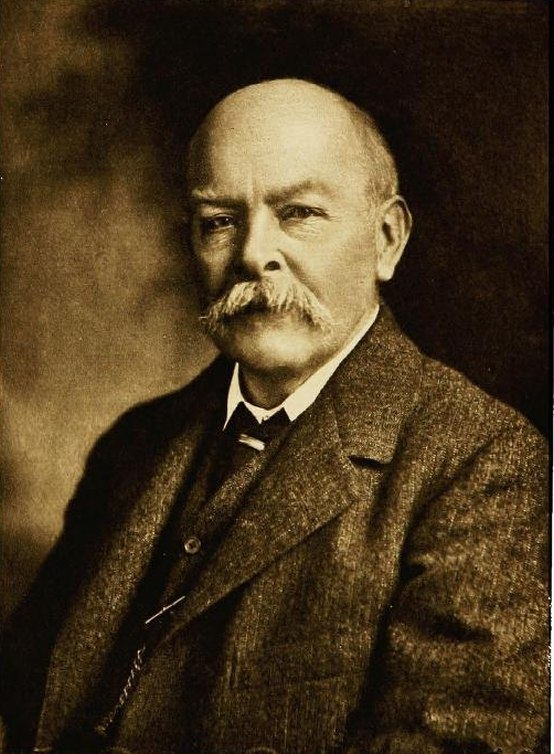
\includegraphics[scale = 0.5]{John_Henry_Poynting.jpg}
\end{figure} 

\begin{figure}[h]
    \centering 
    
\includegraphics[scale = 0.2]{John_Henry_Poynting_signature.png}
\end{figure} 

\newpage 

\section{Teorema di Poynting} 

\footnote{FWC - pag 139 | 3.12 Power flow in electromagnetic fields: Poynting's theorem }

Le onde elettromagnetiche possono portare energia. \\ 

Partendo dalle leggi di Maxwell generali: \\ 

{\Large \begin{equation}
    \begin{cases}
        \nabla \times \vec{E} = - \frac{\partial \vec{B}}{\partial t} \\ 
        \nabla \times \vec{H} = \vec{J} + \frac{\partial \vec{D}}{\partial t}
    \end{cases}
\end{equation}}

Ricordando anche che: \\ 

{\Large \begin{equation}
    \begin{cases}
        \vec{D} = \varepsilon\vec{E} \\ 
        \vec{B} = \mu \vec{H} 
    \end{cases}
\end{equation}} 

Possiamo scrivere, applicando la proprietà dei vettori: 

{
    \Large
    \begin{equation}
    \nabla \cdot (\vec{E} \times \vec{H}) = \vec{H} \cdot (\nabla \times \vec{E}) - \vec{E} \cdot (\nabla \times \vec{H})     
    \end{equation}
}

\begin{tcolorbox}
    Per approfondire questa proprietà vettoriale, puoi consultare questa pagina sul prodotto misto \\
    \url{https://it.wikipedia.org/wiki/Prodotto_misto}
\end{tcolorbox}

Sviluppando i prodotti vettoriali, avremo:  

{
    \Large
    \begin{equation}
    \nabla \cdot (\vec{E} \times \vec{H}) = - \vec{H} \cdot \frac{\partial \vec{B}}{\partial t} - \vec{E} \cdot \frac{\partial \vec{D}}{\partial t} - \vec{E} \cdot \vec{J}       
    \end{equation}
}

Da forma vettoriale a forma integrale: 

{
    \Large
    \begin{equation}
        - \int_V \nabla \cdot (\vec{E} \times \vec{H}) dV = 
        \int_V (\vec{H} \cdot \frac{\partial \vec{B}}{\partial t} + \vec{E} \cdot \frac{\partial \vec{D}}{\partial t} + \vec{E} \cdot \vec{J}) dV
    \end{equation}
}

\begin{tcolorbox}
    
    $\int_V dV$ si chiama integrale di un volume. È come l'integrale visto in analisi matematica 1 a una dimensione, 
    ma applicato in un volume. È un argomento di analisi matematica 2 \\   
    
    Per approfondire questo argomento,  consiglio questo video di \\ \\ 
    Clear Math -  Dall'astratto alla Realtà: guida completa sugli Integrali Tripli per Analisi 2 \\ 
    \url{https://youtu.be/4pDVpcJmnfY?si=pyKpC62rKZrk-i3L} \\ 

    Inoltre, se vuoi capire come siamo passati dalla forma vettoriale $\nabla \cdot (\vec{E} \times \vec{H})$ 
    alla forma integrale $- \int_V \nabla \cdot (\vec{E} \times \vec{H}) dV$, consiglio di vedere questo video 
    sul Teorema di Stokes:  \\ \\ 
    Clear Math - Devi saper fare questo esercizio sul Teorema di Stokes se vuoi passare Analisi 2 \\ 
    \url{https://youtu.be/-r8Er68ZOFk?si=8XxzHIWmG_z9Hl79}

    
    
\end{tcolorbox} 

Dal Teorema della divergenza, sappiamo che, dato un vettore $\vec{F}$: \\ 

{
    \Large 
    \begin{equation}
    \int_V \nabla \cdot \vec{F} dV = \oint_S \vec{F} \cdot \vec{dS}       
    \end{equation}
}

dove $\oint_S \vec{F} \cdot \vec{dS}$ è un integrale di linea lungo una superficie chiusa. \\ \\ 

Quindi, applicando il Teorema della divergenza, possiamo scrivere la precedente equzione come: \\ 

{
    \Large
    \begin{equation}
    - \oint_S (\vec{E} \times \vec{H}) \cdot \vec{dS} = \int_V  (\vec{H} \cdot \frac{\partial \vec{B}}{\partial t} + \vec{E} \cdot \frac{\partial \vec{D}}{\partial t} + \vec{E} \cdot \vec{J}) dV     
    \end{equation}
}

Quest'ultima equazione è il teorema di Poynting per qualsiasi mezzo. \\

Per mezzi lineari che non cambiano nel tempo, il teorema di Poynting lo possiamo scrivere in questa forma: 
{
    \Large
    \begin{equation}
    - \oint_S (\vec{E} \times \vec{H}) \cdot \vec{dS} = \int_V [\frac{\partial}{\partial t} (\frac{\vec{B} \cdot \vec{H}}{2}) + \frac{\partial}{\partial t} (\frac{\vec{D} \cdot \vec{E}}{2}) + \vec{E} \cdot \vec{J} ] dV       
    \end{equation}
}

Sostituendo dalla definizione di $\vec{D}$ e $\vec{B}$ per mezzi lineari in assenza di cariche: 
{
    \Large
    \begin{equation}
        \begin{cases}
\vec{D} = \varepsilon \vec{E}\\ 
\vec{B} = \mu \vec{H}         
        \end{cases}
    \end{equation}
}

L'equazione precedente diventa: 
{
    \Large
    \begin{equation}
    - \oint_S (\vec{E} \times \vec{H}) \cdot \vec{dS} = \int_V \vec{E} \cdot \vec{J} dV + \frac{1}{2} \frac{\partial}{\partial t} [\int_V \varepsilon \left| E \right| ^{2} dV + \int_V \mu \left| H \right| ^{2} dV ]        
    \end{equation}
} 

\begin{tcolorbox}
    $\left| E \right|$ e $\left| H \right|$ rappresentano il modulo, detta anche lunghezza , rispettivamente, del vettore $\vec{E}$ e del vettore $\vec{H}$ \\
    Per approfondire \url{https://www.youmath.it/lezioni/algebra-lineare/matrici-e-vettori/691-vettori-e-versori.html}
\end{tcolorbox} 

Quindi, $- \oint_S (\vec{E} \times \vec{H}) \cdot \vec{dS} $ rappresenta l'energia che entra in un volume per unità di tempo. \\ \\
In notazione matematica: 
{   
    \Large
    \begin{equation}
    W = \oint_S \vec{P} \cdot \vec{dS}      
    \end{equation}
}

dove: 

{   
    \Large
    \begin{equation}
    \vec{P} = \vec{E} \times \vec{H}        
    \end{equation}
}

è chiamato il vettore Poynting.  \\

Dalla definizione di prodotto vettoriale, sappiamo che: 
{
    \Large
    \begin{equation}
  \vec{E} \times \vec{H} = \left|E\right| \left|H\right| \sin(\theta)      
    \end{equation}
}

dove $\theta$ (si legge theta), è l'angolo compreso tra $\vec{E}$ e $\vec{H}$ \\ \\ 

$\left|P\right| = 0$ quando $\left|E\right|$ e/o $\left|H\right|$ = 0, oppure quando 
$\vec{E} \parallel \vec{H}$ (si legge vettore E parallelo a vettore H) perchè $\theta = 180 ^{\circ} \rightarrow \sin(180^{\circ}) = 0$ sempre. \\ \\ 

Inoltre, in un conuttore perfetto, $\left|P\right| = 0$ sempre, perchè, in un conduttore perfetto, la componente tangenziale di $\vec{E}$ è uguale a zero. \\ \\ 

\newpage 


\section{Perdite Ohmiche} 

\footnote{ FWC - pag 141 | Example 3.12a Ohmic loss} 

Dato un conduttore cilindrico, possiamo avere $I_z$ come corrente lungo l'asse z. \\ 
Se R è la resistenza per dZ, allora, utilizzando la legge di Ohm, avremo che: 
{
    \Large
    \begin{equation}
    E_z = I_z R     
    \end{equation}
}

H è in una superficie radiale, fuori dal cilindro. Per un raggio r, possiamo esprime $H_\phi$ come: 

{
    \Large
    \begin{equation}
    H_\phi = \frac{I_z}{2\pi r}     
    \end{equation}
}

Usando il teorema di Poynting, $\vec{P} = \vec{E} \times \vec{H}$, quindi: 
{
    \Large
    \begin{equation}
    P_r = -E_z H_\phi = - \frac{R I_z^{2}}{2\pi r}        
    \end{equation}
}

Ora possiamo integrare per la superficie chiusa, che in questo caso è un cerchio, in cui l'incognita è 
il raggio e avremo che: 

{
    \Large
    \begin{equation}
    W = 2\pi r (-P_r) = I_z ^{2} R        
    \end{equation}
}

Grazie a questo esempio, possiamo pensare al vettore Poynting come la densità 
di flusso di potenza in un punto.  

\begin{figure}[h]
    \centering 
    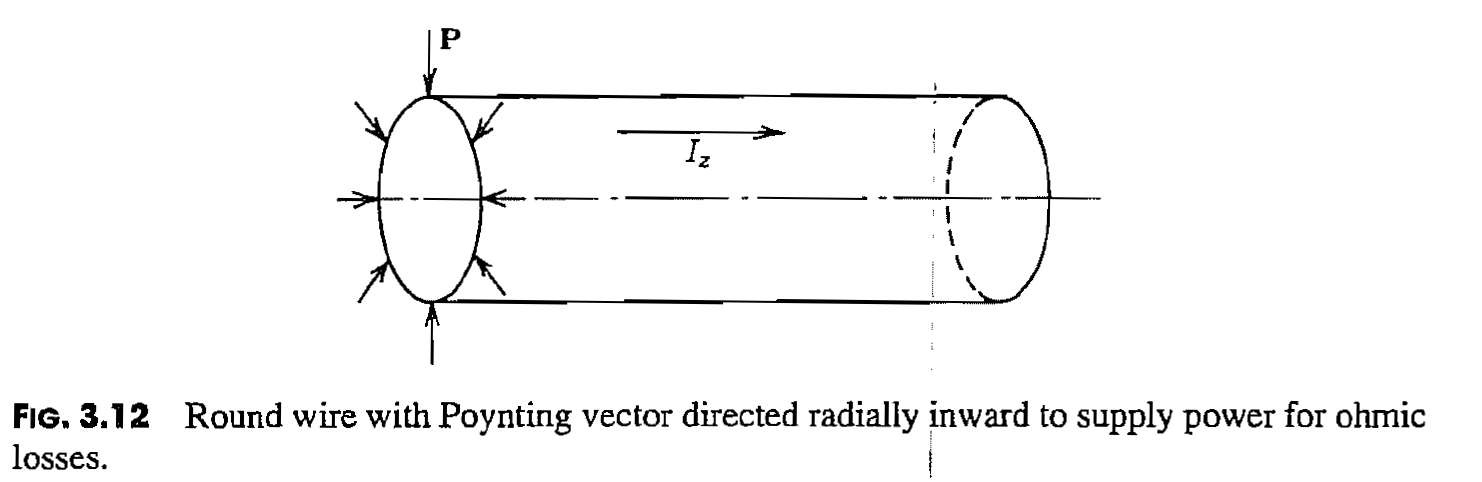
\includegraphics[scale = 0.5]{Ohmic loss.PNG} 
    
\end{figure}  

\footnote{FWC pag 142 } 

\newpage 

\section{Teorema di Poynting per un'onda piana}

\footnote{FWC - pag 143 | Example 3.12c Poynting flow in a plane wave} 

Data un'onda piana sinusoidale che varia in x e y con: 

{
    \Large
    \begin{equation}
        \begin{cases}
            E_x = E_o \cos(\omega t - \kappa z) \\
            H_y = \sqrt{\frac{\varepsilon}{\mu}} E_o \cos(\omega t - \kappa z)                         
        \end{cases}
    \end{equation}
}

che si propaga nella direzione z. \\

Dal teorema di Poynting: 
{
    \Large
    \begin{equation}
        \begin{split}
        \vec{P} 
        &= \vec{E} \times \vec{H} 
        \\ 
        &= \left|E_x\right| \left|H_y\right| \sin(\theta) 
        \end{split}
    \end{equation}
}

Essendo 
{
    \Large
    \begin{equation}
   \theta = 90 ^{\circ} 
   \rightarrow \sin(\theta) = 1     
    \end{equation}
} 

quindi: \\ 

{
    \Large
    \begin{equation}
        \begin{split}
            P_z 
            &= E_x H_y 
            \\
            &= \sqrt{\frac{\varepsilon}{\mu}} E_o ^{2} \cos^{2}(\omega t - \kappa z) 
            \\
            &= \frac{E_o ^{2}}{\eta } \cos^{2}(\omega t - \kappa z)        
        \end{split}
    \end{equation}
}

Utilizzando l'identità trigonometrica: 

{
    \Large
    \begin{equation}
    \sin^{2}(x) + \cos^{2}(x) = 1     
    \end{equation}
}

$P_z$ sarà:  

{
    \Large
    \begin{equation}
        \begin{split}
        P_z 
        &= 
        \sqrt{\frac{\varepsilon}{\mu}} E_o ^{2} [\frac{1}{2} + \frac{1}{2} \cos 2 (\omega t - \kappa z)] 
        \\ 
        &= \frac{E_o ^{2}}{\eta} [\frac{1}{2} + \frac{1}{2} \cos 2 (\omega t - \kappa z)]
        \end{split}
    \end{equation}
}

\begin{tcolorbox}
    Negli esercizi di esame, quando viene data la potenza dell'onda, il termine \\ $[\frac{1}{2} + \frac{1}{2} \cos 2 (\omega t - \kappa z)] = 0$, quindi \\ 

    $P_z = \frac{1}{2} \sqrt{\frac{\varepsilon}{\mu}} E_o ^{2} = \frac{E_o ^{2}}{2 \eta}$


\end{tcolorbox}

\newpage 

\section{Teorema di Poynting per i fasori} 

\footnote{FWC - pag 143 | 3.13 Poynting's theorem for phasors} 

Rispetto all'equazione di Maxwell in forma fasoriale, non possiamo sostituire $\jmath \omega$ a $\frac{\partial}{\partial t}$ per il 
Teorema di Poynting, quindi procediamo per step. \\ \\ 

Prendendo le equazione di Maxwell nella loro forma generale per i fasori: \\ 

{\Large \begin{equation}
    \begin{cases}
        \nabla \times \vec{E} = - \jmath \omega \vec{B} \\ 
        \nabla \times \vec{H} = \vec{J} + \jmath \omega \vec{D}
    \end{cases}
\end{equation}}

in cui, ricordiamo che: 

{
    \Large
    \begin{equation}
        \begin{cases}    
\vec{D} = \varepsilon \vec{E} 
\\
\vec{B} = \mu \vec{H}        
        \end{cases}
    \end{equation}
}

Consideriamo l'identità vettoriale: 

{
    \Large
    \begin{equation}
    \nabla \cdot (\vec{E}  \times \vec{H}^{*}) = \vec{H} ^{*} \cdot (\nabla \times \vec{E}) - \vec{E} \cdot (\nabla \times \vec{H} ^{*})        
    \end{equation}
}

dove l'asterisco denota il vettore complesso coniugato. 

\begin{tcolorbox}
    Dalla matematica, il vettore complesso coniugato è il vettore che ha lo stesso modulo del vettore originale, ma 
    verso opposto della parte immaginaria. \\ 

    Se vuoi approfondire: \\ \url{https://www.youmath.it/lezioni/analisi-matematica/numeri-complessi/3504-complesso-coniugato.html}


\end{tcolorbox}  

Applicando le equazioni di Maxwell in forma generale per i fasori, avremo che: 
{
    \Large
    \begin{equation}
    \nabla \cdot (\vec{E} \times \vec{H}^{*}) = \vec{H}^{*} \cdot (- \jmath \omega \vec{B}) - \vec{E} \cdot (\vec{J}^{*} - \jmath \omega \vec{D}^{*})      
    \end{equation}
}

Integrando entrambi i membri per un volume V e applicando il teorema della divergenza a entrambi i membri dell'equazione, avremo che: \\ 

{\Large \begin{equation}
    \begin{split}
        \int_V \nabla \cdot (\vec{E} \times \vec{H}^{*}) dV 
        &= \oint_S (\vec{E} \times \vec{H}^{*}) \cdot \vec{dS} 
        \\
        &= - \int_V [\vec{E} \cdot \vec{J}^{*} + \jmath \omega (\vec{H}^{*} \cdot \vec{B} - \vec{E} \cdot \vec{D}^{*})] dV       
    \end{split}
\end{equation}}

Questa è l'equazione generale del teorema Poynting in forma fasoriale. \\ \\ 

Sapendo che in un mezzo lineare isotropico 
{
    \Large
    \begin{equation}
    \vec{J} = \sigma \vec{E}         
    \end{equation}
}

e che $\sigma$, $\mu$ e $\varepsilon$ sono scalari, 
possiamo riscrivere il teorema di Poynting in forma fasoriale come: \\ 

{\Large \begin{equation}
    \oint_S (\vec{E} \times \vec{H}) \cdot dS = - \int_V \sigma \vec{E} \cdot \vec{E}^{*} dV - \jmath \omega \int_V [\mu \vec{H} \cdot \vec{H}^{*} - \varepsilon \vec{E} \cdot \vec{E}^{*}] dV
\end{equation}}

$- \int_v \sigma \vec{E} \cdot \vec{E}^{*} dV $ rappresenta il doppio della potenza media che si perde in un conduttore 
di corrente, quindi la potenza media è: 

{\Large \begin{equation}
    P_{av} = \frac{1}{2} \Re(\vec{E} \times \vec{H}^{*})
\end{equation}}


$P_{av}$ si misura in $[\frac{W}{m^2}]$ \\ (si legge Watt per metro quadro)  \\ \\ 

Per un mezzo lineare isotropico:

{
    \Large
    \begin{equation}
    - \jmath \omega \int_V [\mu \vec{H} \cdot \vec{H}^{*} - \varepsilon \vec{E} \cdot \vec{E}^{*}] dV = -\jmath \omega \int_V \frac{1}{2} [\frac{1}{2} \varepsilon \left|E\right|^{2} - \frac{1}{2} \mu \left|H\right|^{2} ] dV    
    \end{equation}
}

Allora: 
{\Large \begin{equation}
    \Im\oint_S (\vec{E} \times \vec{H}^{*}) \cdot \vec{dS} = 4\omega (U_{Eav} - U_{Hav})
\end{equation}}

dove $U_{Eav}$ e $U_{Hav}$ sono rispettivamente l'energia immagazzinata di campo elettrico e di campo magnetico. \\ \\ 

Quindi, la parte immmaginaria del teorema di Poynting può essere vista come la potenza reattiva, cioè la potenza opposta 
alla direzione di propagazione dell'onda. 

\newpage 

\section{Potenza media in un'onda piana uniforme} 

\footnote{FWC - pag 145 | Example 3.13 Average power in uniform plane waves} 

Considerando le onde piane scritte in forma fasoriale: 

{\Large \begin{equation}
    \begin{cases}
        E_x = C_1 e^{-\jmath \kappa z} + C_2 e^{\jmath \kappa z} \\ 
        H_y = \sqrt{\frac{\varepsilon}{\mu}} [C_1 e^{-\jmath \kappa z} + C_2 e^{\jmath \kappa z}] 
    \end{cases}
\end{equation}}

\begin{tcolorbox}
    L'onda qui indicato è polarizzata linearmente per $E_x$. \\ 
    La polazizzione è un argomento che andremo ad affrontare in un capitolo futuro. 
\end{tcolorbox}


Il vettore Poynting in forma complessa è: 

{\Large \begin{equation}
    \vec{E} \times \vec{H} = \sqrt{\frac{\varepsilon}{\mu}} [C_1 e^{-\jmath \kappa z} + C_2 e^{\jmath \kappa z}] [C_1^{*} e^{-\jmath \kappa z} + C_2^{*} e^{\jmath \kappa z}] \hat{z}
\end{equation}}

Quindi, la potenza media lungo la direzione z è: 

{\Large \begin{equation}
    P_{av} = \frac{1}{2} \sqrt{\frac{\varepsilon}{\mu}} [C_1 C_1^{*} - C_2 C_2^{*}]
\end{equation}}

$P_{av}$ esprime che la potenza media lungo z è uguale alla potenza dell'onda lungo z sottratto alla potenza 
dell'onda lungo -z. \\ \\ 

\newpage 

